\chapter{Comment utiliser l'application ?}

Cette application se nomme \textbf{Chronos}, et vous permet de configurer des alarmes en conversant avec un agent. Pour que l'agent accepte de configurer votre alarme, vous devrez fournir une date ainsi qu'une heure lors de votre échange avec ce dernier. 

Si vous êtes satisfait de l'alarme que vous voulez configurer, alors vous
aurez la possibilité de le confirmer et l'agent programmera ainsi cette alarme, qui, lors de son déclenchement, sera accompagnée d'une musique relative à la météo liée à votre géolocalisation. 

~\\\indent \textbf{Attention :} Pour le moment, pour qu'une alarme se déclenche, il ne faut pas tuer l'application et la laisser tourner en tâche de fond.

\section{Pré-requis}
Nous supposerons que vous posséder un \emph{SmartPhone} avec une version d'Android supérieure à \texttt{4.2.x}. Vous devez également avoir installé l'application
en suivant le \textbf{manuel d'installation}.\\

Dans la suite de ce manuel, vous retrouverez les icônes en figures \ref{hand} et \ref{voice} qui vous donneront des informations.

\begin{figure}[H]
  \centering
  
\includegraphics[width=2cm]{images/hand.png}
  \caption{Cette icône vous indique soit un endroit où cliquer à l'écran de votre \emph{SmartPhone}, soit attire votre attention sur un détail en particulier.}
  \label{hand}
\end{figure}

\begin{figure}[H]
  \centering
  
\includegraphics[width=2cm]{images/voice.png}
  \caption{Cette icône vous indique que vous devez parler dans le microphone de votre \emph{SmartPhone}.}
  \label{voice}
\end{figure}

\section{Ouverture de l'application}

Vous pouvez ouvrir l'application en cliquant dessus comme sur la figure \ref{A}.

\begin{figure}[H]
  \centering
  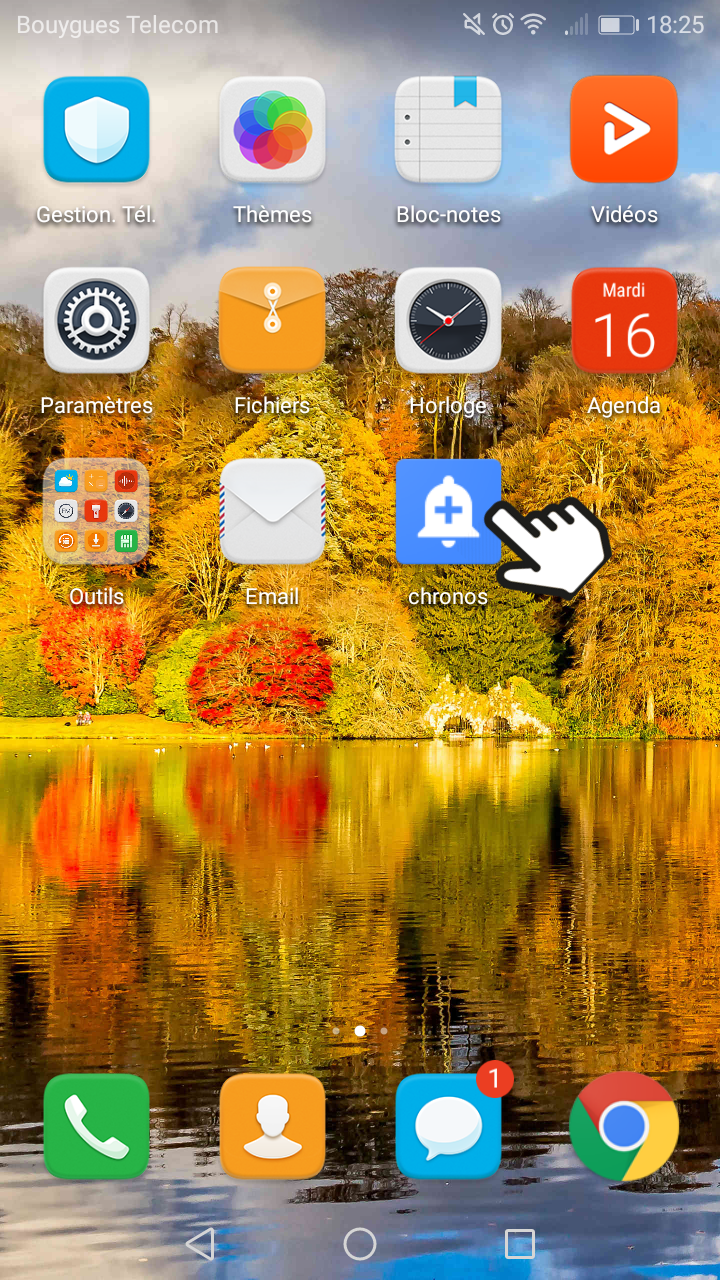
\includegraphics[width=6cm]{images/A.png}
  \caption{Ouverture de l'application}
  \label{A}
\end{figure}

\begin{figure}[H]
  \centering
  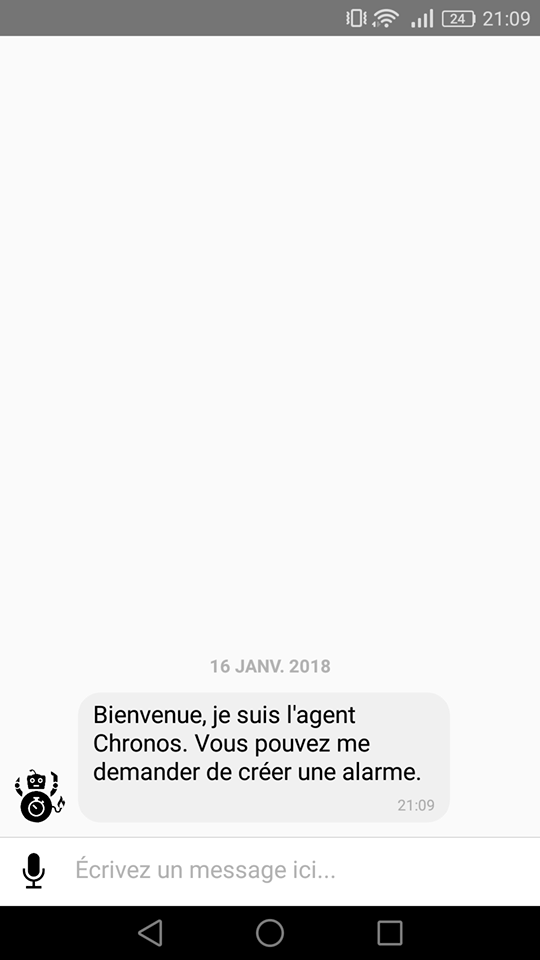
\includegraphics[width=6cm]{images/B1.png}
  \caption{Ecran principal}
  \label{B1}
\end{figure}

Une fois l'application ouverte, vous tombez sur l'écran représenté en figure \ref{B1}. Vous pouvez communiquer avec l'agent \emph{via} le microphone en appuyant une fois sur l'icône de micro
ou directement en entrant le texte dans le champ texte se situant à coté de l'icône de micro. 

~\\\indent Vous n'êtes pas obligé de donner à l'agent l'ensemble des données
dont il a besoin pour configurer votre alarme \--- en effet vous pouvez très bien y aller étape par étape comme nous allons le voir. 

~\\\indent Vous pouvez commencer par cliquer
une fois sur l'icône micro et dire que vous désirez mettre une alarme (figures \ref{B} et \ref{C}).

\begin{figure}[H]
  \centering
  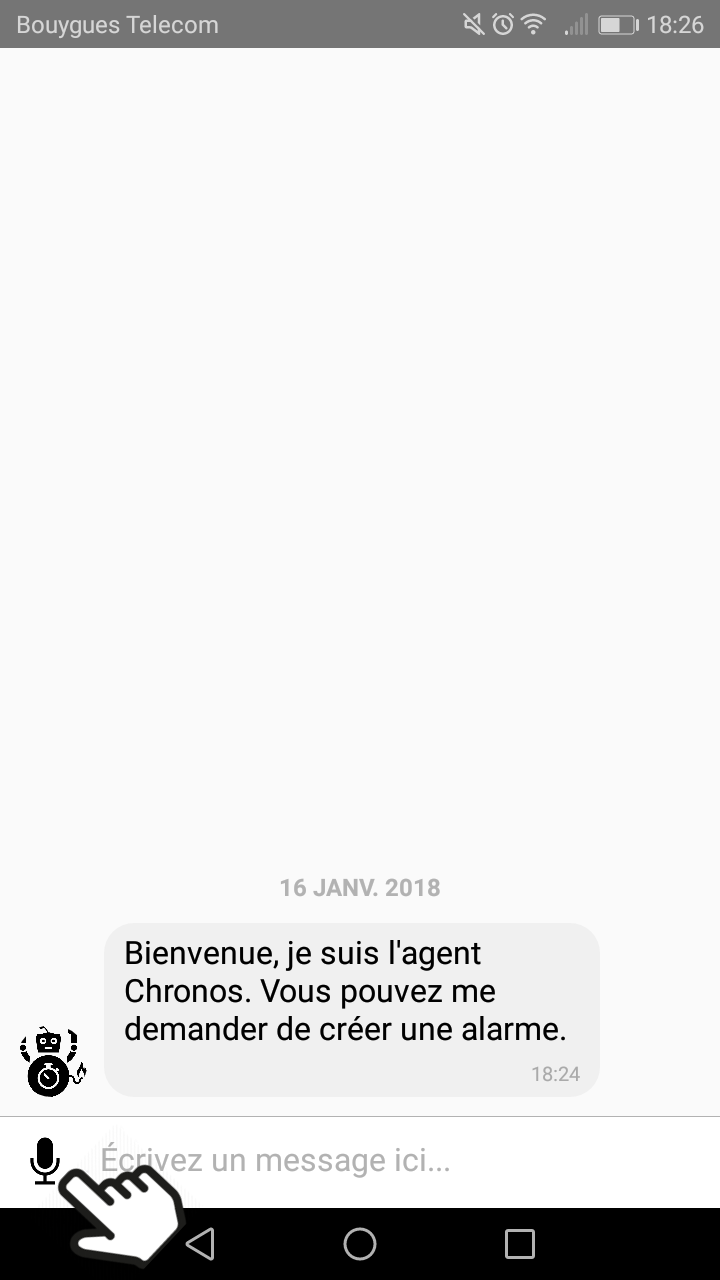
\includegraphics[width=6cm]{images/B.png}
  \caption{Cliquer sur l'icône micro}
  \label{B}
\end{figure}

\begin{figure}[H]
  \centering
  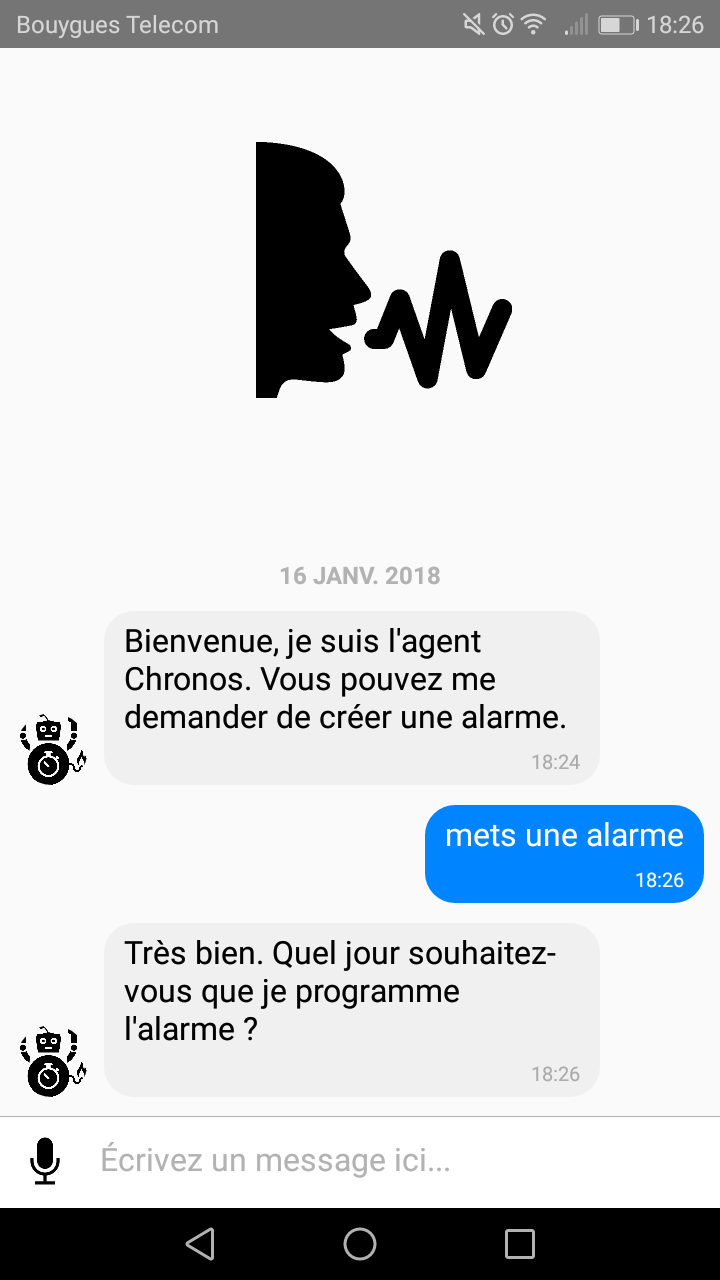
\includegraphics[width=6cm]{images/C.png}
  \caption{Demander la programmation d'une alarme avec la voix}
  \label{C}
\end{figure}

L'application détectera automatiquement que vous avez cessé de parler, vous n'avez donc pas besoin de ré-appuyer sur l'icône micro pour signaler la fin de votre phrase.

~\\\indent Ensuite, vous pouvez indiquer la date à laquelle déclencher l'alarme en cliquant de nouveau sur l'icône micro (figure \ref{D}).

\begin{figure}[H]
  \centering
  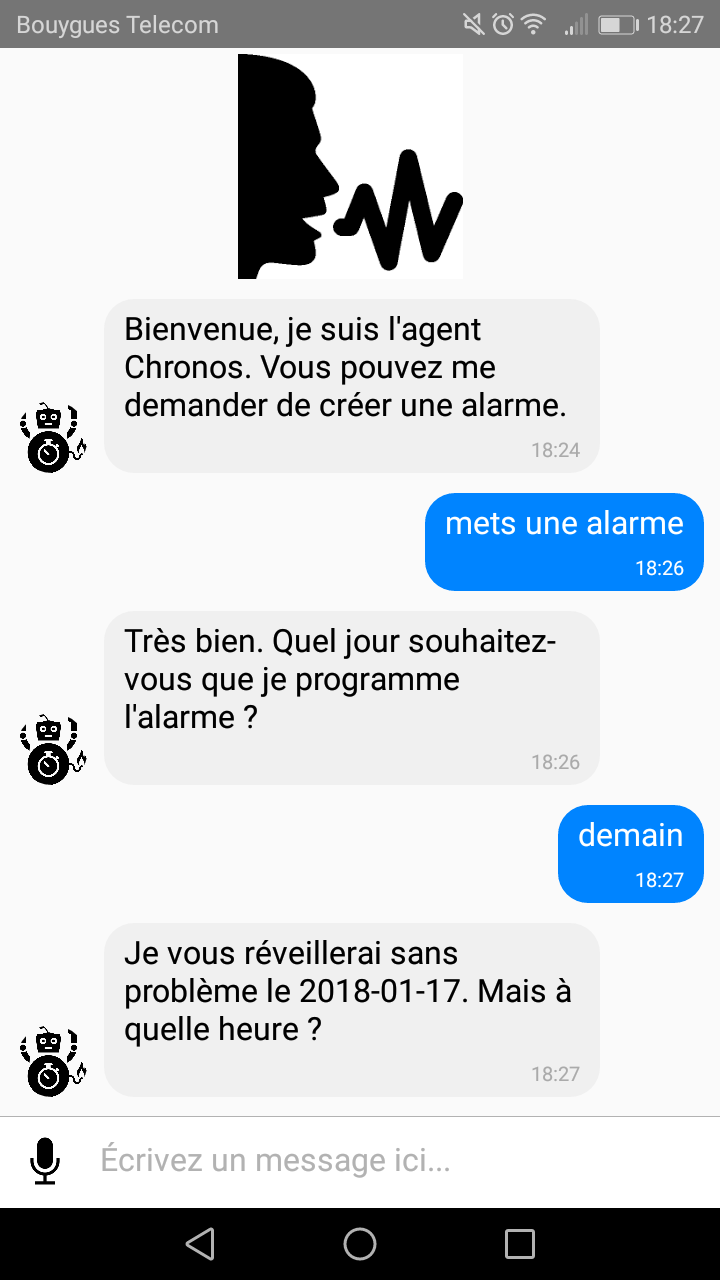
\includegraphics[width=6cm]{images/D.png}
  \caption{Indiquer la date avec la voix}
  \label{D}
\end{figure}

Puis pour finir en lui indiquant l'heure à laquelle déclencher l'alarme. 

~\\\indent S'il a bien reconnu votre intention, l'agent vous demandera ensuite une confirmation comme l'illustre la figure \ref{E}.

\begin{figure}[H]
  \centering
  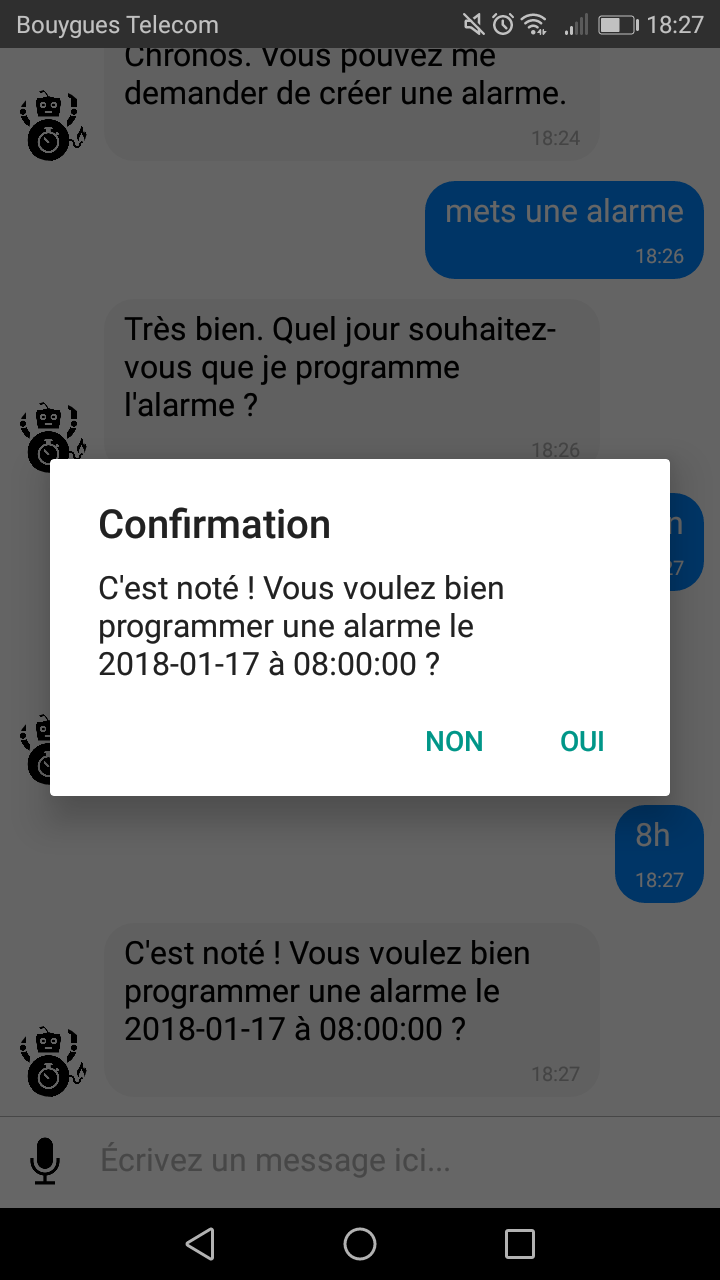
\includegraphics[width=6cm]{images/E.png}
  \caption{Indiquer l'heure et écran de confirmation}
  \label{E}
\end{figure}


Vous auriez très bien pu converser avec l'agent via l'entrée textuelle, comme le représente la figure \ref{F}.

\begin{figure}[H]
  \centering
  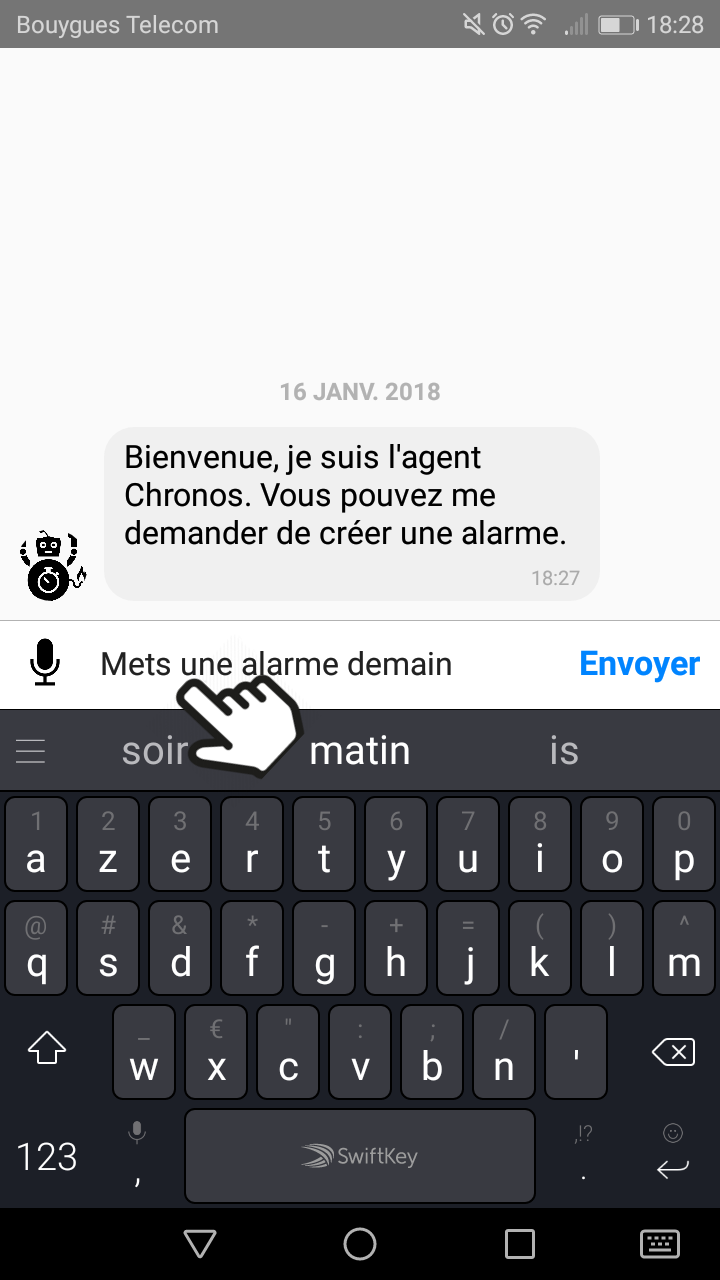
\includegraphics[width=6cm]{images/F.png}
  \caption{Demande de programmation d'une alarme \emph{via} texte}
  \label{F}
\end{figure}

Si vous avez confirmé la programmation de l'alarme, l'agent enregistrera votre demande. Une minute avant le déclenchement de l'alarme demandée, il vous indiquera la météo associée à votre géolocalisation. 

~\\\indent
Comme le montre la figure suivante, vous pouvez également programmer l'alarme en une seule phrase si celle-ci est complète (figure \ref{G}).

\begin{figure}[H]
  \centering
  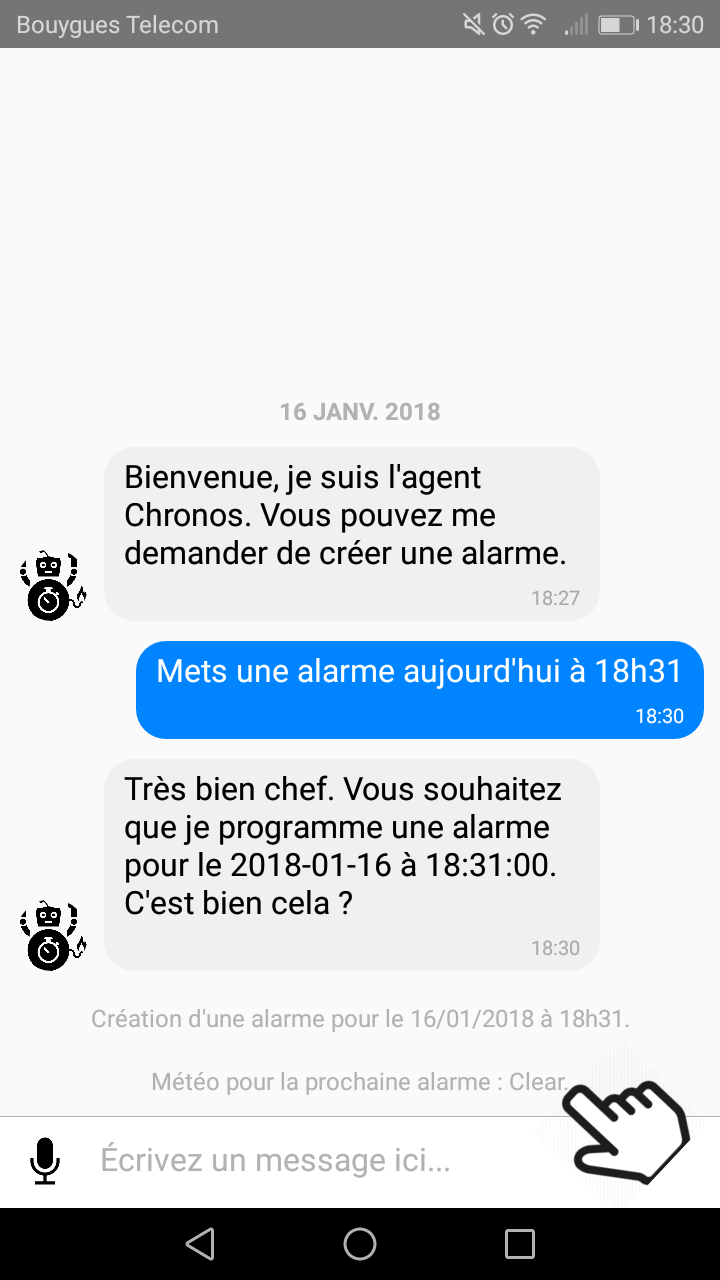
\includegraphics[width=6cm]{images/G.png}
  \caption{Météo associée à l'alarme}
  \label{G}
\end{figure}

Lorsque qu'une alarme se déclenchera, vous recevrez une notification accompagnée de la musique associée à la météo liée à votre localisation (figure \ref{H}).

\begin{figure}[H]
  \centering
  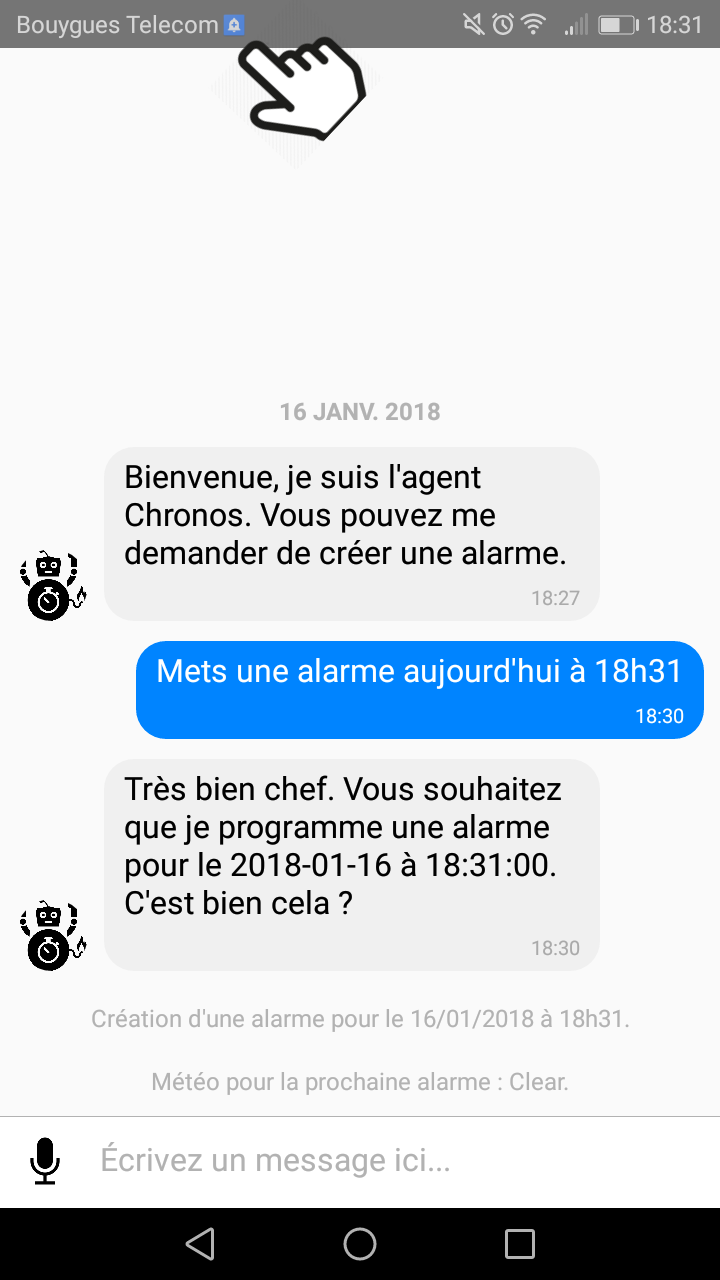
\includegraphics[width=6cm]{images/H.png}
  \caption{Déclenchement d'une alarme : notification}
  \label{H}
\end{figure}

~\\\indent
\textbf{Petit bonus :} l'agent reconnaîtra quelques phrases supplémentaires non liées aux fonctionnalités prévues initialement pour l'application (figure \ref{J}), à vous de les découvrir \textsf{;)}.

\begin{figure}[H]
  \centering
  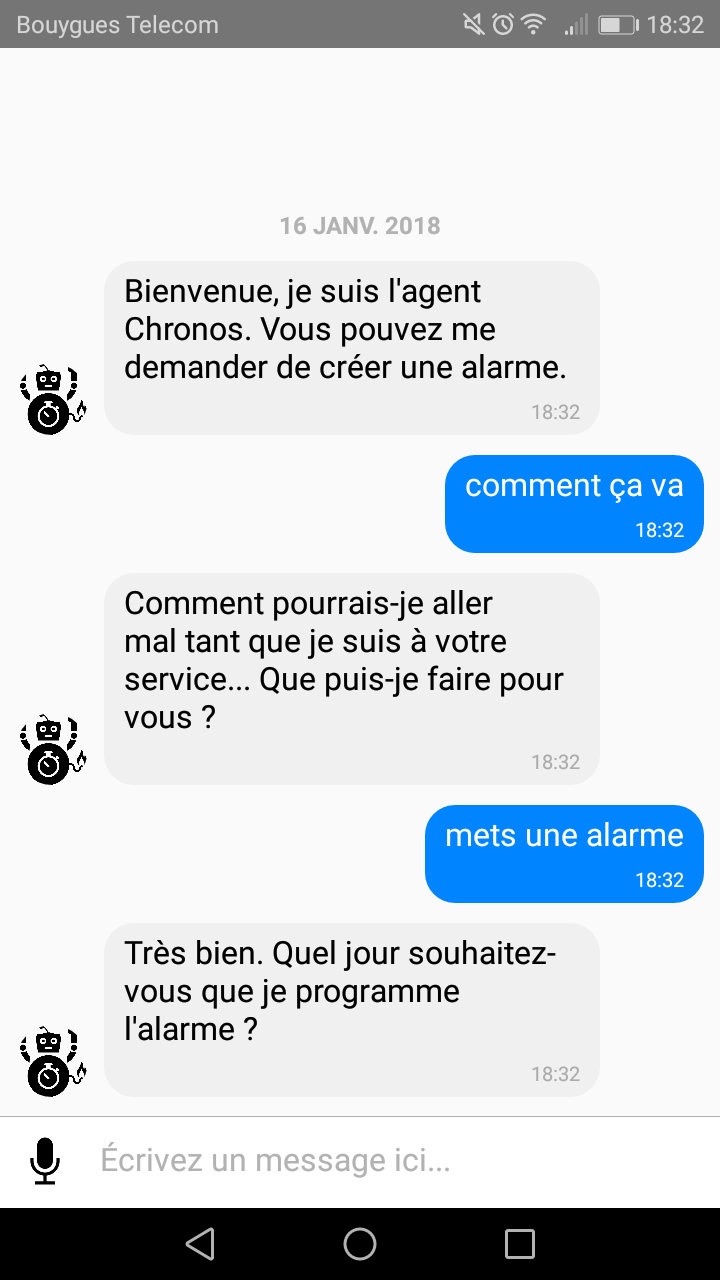
\includegraphics[width=6cm]{images/J.png}
  \caption{Petite conversation bonus}
  \label{J}
\end{figure}
